\section{Results}\label{results}

Submissions to the ArgMining~2021 shared task on Quantitative Summarization and Key Point Analysis are evaluated with respect to mean average precision~(mAP).\footnote{\url{https://2021.argmining.org/shared_task_ibm.html}}
%\todo{Cite the task overview paper once the citation is announced.}
The organizers calculate the score by pairing each argument with the best matching key point according to the predicted matching probabilities.
Within each topic-stance combination, only the 50\,\% of arguments with the highest predicted matching score are then considered for evaluation.
The task organizers claim that this removal of 50\,\% of the pairs is sensible because some arguments do not match any of the key points, which would influence mean average precision negatively. % \todocite
For the remaining argument key point pairs in each topic-stance combination, average precision is calculated and the final score is computed as the mean of all average precision scores.

The task organizers now consider two variants of ground-truth labels: strict labels and relaxed labels.
Both variants are based on the ground-truth labels from the ArgKP dataset~\cite{Bar-HaimEFKLS2020}. But as the ArgKP dataset contains argument key point pairs with undecided labels~(i.e. not enough agreement between annotators), the shared task organizers derive strict labels by considering those pairs as no match, and relaxed labels by considering them as match. % \todocite
To compute each evaluation score, the strict score is calculated based on strict ground-truth labels and the relaxed score is calculated based on relaxed ground-truth labels. % \todocite

We stress that in the complex evaluation setup of the mean average precision score, the relaxed mAP score would favor assuming matches in case of model uncertainty while the strict mAP on the opposite would favor assuming no match.
Though, as only the most-probable matching key point is being considered for evaluation, this effect is minor.
The evaluation score in general favors matchers that can match a single key point for each argument with high precision.
It is however not important if a matcher does predict non-matches with high certainty.

\subsection{Discussion}
\begin{table*}
  \centering
  \caption{Performance of the random and token overlap baseline, \BertBase, and \RobertaBase models with respect to mean average precision~(mAP), precision, and recall of the match label. We report scores for the training, validation, and test set in the strict~(S) and relaxed~(R) label settings, as well as the averages of the two settings~(\(\varnothing\)). The best result per set is highlighted \textbf{bold}.}
  \label{table-results}
  \smaller
  \setlength{\tabcolsep}{2.5mm}
  \begin{tabularx}{\linewidth}{X>{\hspace{1.0em}}ccc<{\hspace{1.0em}}>{\hspace{1.0em}}ccc<{\hspace{1.0em}}>{\hspace{1.0em}}ccc}
    \toprule
    \textbf{Approach} & 
    \multicolumn{3}{c}{\textbf{mAP}} & 
    \multicolumn{3}{c}{\textbf{Precision}} & 
    \multicolumn{3}{c}{\textbf{Recall}} \\
    \cmidrule(l{1em}r{1em}){2-4} \cmidrule(l{1em}r{1em}){5-7} \cmidrule(l{1em}){8-10}
    & S & R & \(\varnothing\) & 
    S & R & \(\varnothing\) & 
    S & R & \(\varnothing\) \\
    \midrule
    \multicolumn{10}{X}{\textit{Training set}} \\
    \midrule
    Random & 
    0.260 & 0.409 & 0.335 & 
    0.173 & 0.330 & 0.252 & 
    0.500 & 0.501 & 0.501 \\
    Token Overlap & 
    0.541 & 0.653 & 0.597 & 
    0.269 & 0.435 & 0.352 & 
    0.323 & 0.275 & 0.299 \\
    \BertBase & 
    0.889 & \textbf{0.981} & 0.935 & 
    \textbf{0.703} & \textbf{0.936} & \textbf{0.819} & 
    \textbf{0.864} & \textbf{0.607} & \textbf{0.736} \\
    \RobertaBase & 
    \textbf{0.915} & 0.979 & \textbf{0.947} & 
    0.702 & 0.927 & 0.814 & 
    0.820 & 0.572 & 0.696 \\
    \midrule
    \multicolumn{10}{X}{\textit{Validation set}} \\
    \midrule
    Random & 
    0.232 & 0.430 & 0.331 & 
    0.180 & 0.364 & 0.272 & 
    0.523 & 0.524 & 0.524 \\
    Token Overlap & 
    0.643 & 0.802 & 0.722 & 
    0.219 & 0.416 & 0.317 & 
    0.390 & 0.366 & 0.378 \\
    \BertBase & 
    0.717 & 0.928 & 0.822 & 
    0.397 & 0.648 & 0.522 & 
    \textbf{0.802} & \textbf{0.649} & \textbf{0.725} \\
    \RobertaBase & 
    \textbf{0.879} & \textbf{0.984} & \textbf{0.932} & 
    \textbf{0.567} & \textbf{0.816} & \textbf{0.692} & 
    0.799 & 0.569 & 0.684 \\
    \midrule
    \multicolumn{10}{X}{\textit{Test set}} \\
    \midrule
    Random & 
    0.237 & 0.355 & 0.296 & 
    0.150 & 0.286 & 0.218 & 
    0.545 & 0.549 & 0.547 \\
    Token Overlap & 
    0.483 & 0.575 & 0.529 & 
    0.232 & 0.350 & 0.291 & 
    0.225 & 0.178 & 0.201 \\
    \BertBase & 
    0.827 & 0.940 & 0.883 & 
    0.326 & 0.526 & 0.426 & 
    \textbf{0.848} & \textbf{0.721} & \textbf{0.784} \\
    \RobertaBase & 
    \textbf{0.913} & \textbf{0.967} & \textbf{0.940} & 
    \textbf{0.490} & \textbf{0.716} & \textbf{0.603} & 
    0.741 & 0.569 & 0.655 \\
    \bottomrule
  \end{tabularx}
\end{table*}

In Table~\ref{table-results}, we report mean average precision for strict and relaxed labels of the training, validation, and test set in the ArgKP dataset.
We complement the mAP scores by adding precision, recall, and F1 scores of the match label, both in the strict and relaxed label setting.
To aggregate the results of the strict and relaxed settings we also report the average score of the two variants.
The reported scores should allow for automated and unbiased evaluation of our models and easier comparison with competitive approaches.
We report all 36~scores for the token overlap baseline model as well as for the fine-tuned \BertBase and \RobertaBase models.
To make our results more comparable, we add a second baseline, where matches between arguments and key points of same topic and stance are predicted with uniform random probability.
That random baseline represents a worst-case matcher and any weak matcher should exceed it's evaluation scores.

The token overlap baseline achieves a mean average precision of~0.483 in the strict settings and~0.575 with relaxed labels on the test set.
Thus it is nearly twice as good as a random matcher with respect to mAP.
Even though this baseline has reasonably good scores on all datasets, we are concerned about the large discrepancies between its scores on the validation set and the training and test dataset.
Similarly, the rarher simple baseline is not very robust and thus is prone to variation in performance based on how good the dataset is described by its tokens.

Both fine-tuned matchers outperform the baselines by a large margin.
While the \BertBase matcher achieves a higher relaxed mAP on the training set than the \RobertaBase matcher, the \RobertaBase matcher is overall better than \Bert.
It achieves a mean average precision of 0.913 with strict labels on the test set, and 0.967 with relaxed labels. As these scores are nearly as high on the test set like on the training set, we argue that \Roberta, as a robust language model, generalizes better than \Bert.
Also the \RobertaBase matcher is trained more on precision, while the \BertBase matcher is better with respect to recall for all datasets and strict or relaxed labels.

% \todo{Discuss precision, recall, and F1-score.}

\subsection{Error Analysis}

\begin{figure*}
    \centering
    \begin{subfigure}{0.42\textwidth}
        \centering
        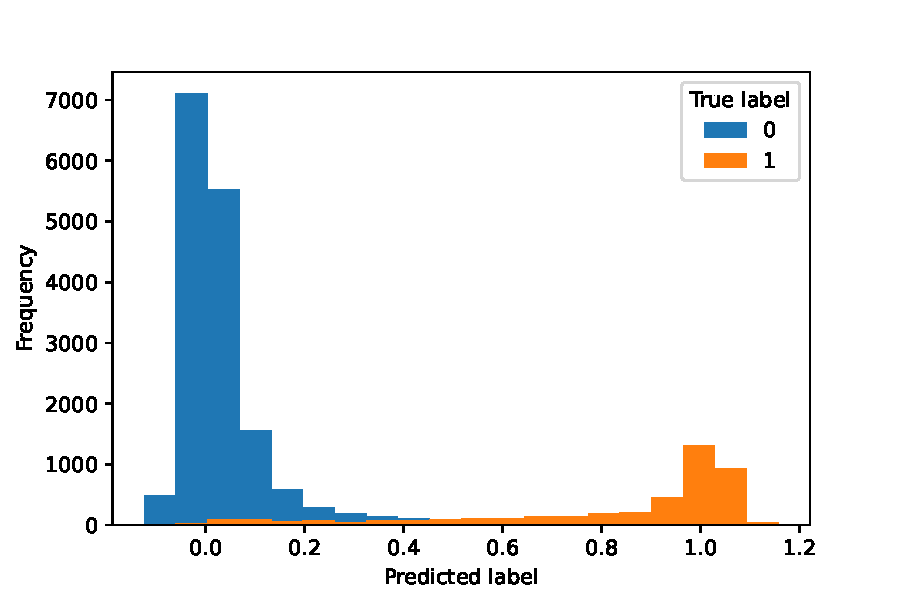
\includegraphics[width=\linewidth]{histogram-labels-bert-train.pdf}
        \subcaption{Predictions with \BertBase on the training set.}
        \label{subfig:bert_train}
    \end{subfigure}
    \hfill
    \begin{subfigure}{0.42\textwidth}
        \centering
        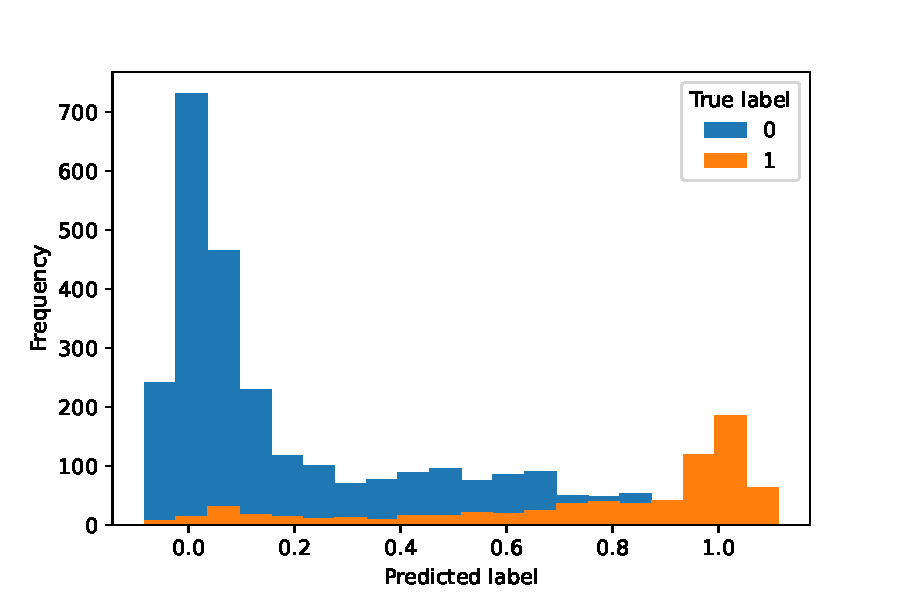
\includegraphics[width=\linewidth]{histogram-labels-bert-dev.pdf}
        \subcaption{Predictions with \BertBase on the validation set.}
        \label{subfig:bert_dev}
    \end{subfigure}
    \begin{subfigure}{0.42\textwidth}
        \centering
        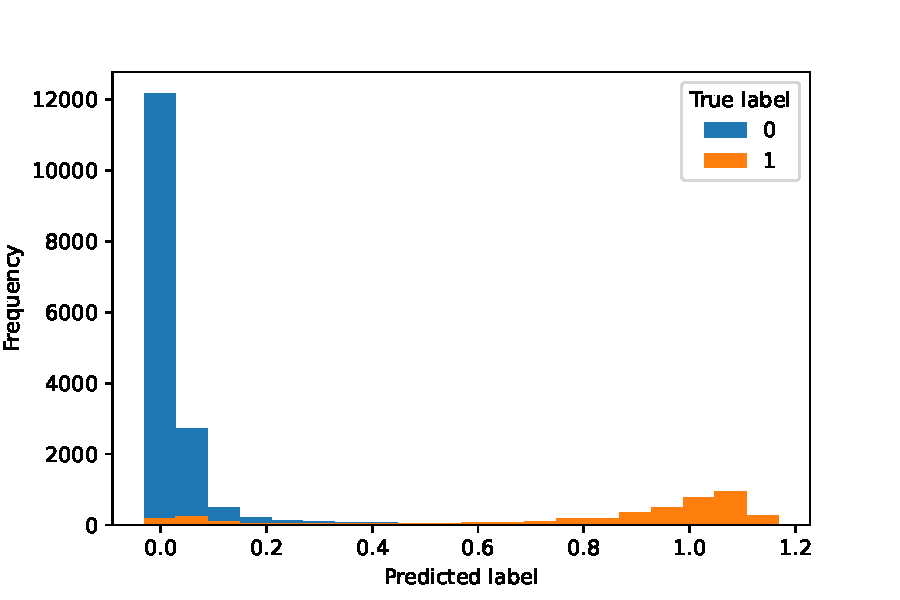
\includegraphics[width=\linewidth]{histogram-labels-roberta-train.pdf}
        \subcaption{Predictions with \RobertaBase on the training set.}
        \label{subfig:roberta_train}
    \end{subfigure}
    \hfill
    \begin{subfigure}{0.42\textwidth}
        \centering
        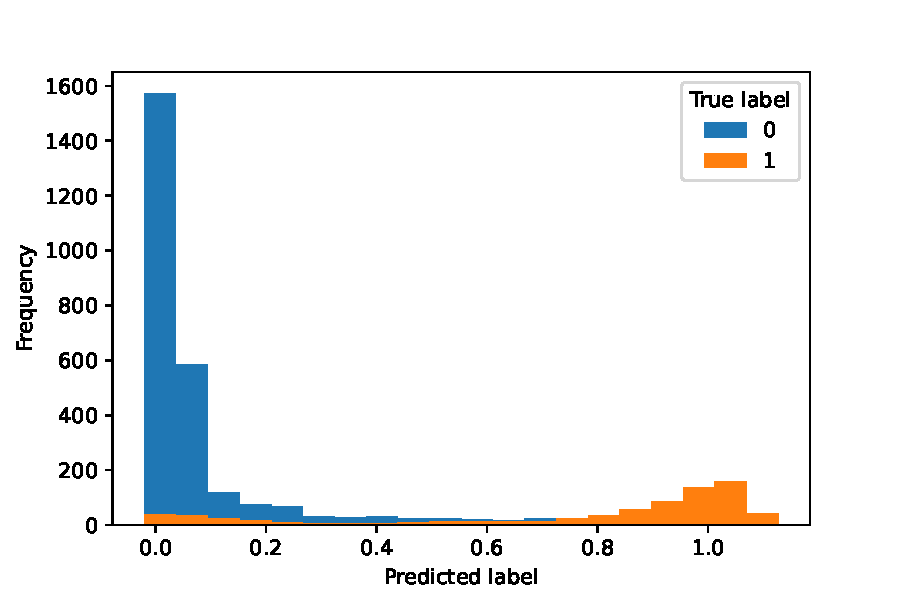
\includegraphics[width=\linewidth]{histogram-labels-roberta-dev.pdf}
        \subcaption{Predictions with \RobertaBase on the validation set.}
        \label{subfig:roberta_dev}
    \end{subfigure}
    \caption{Histograms of predicted labels on the training and validation sets for argument key point pairs with the \BertBase and \RobertaBase classifiers. For good classifiers, predicted labels should approximately equal the true label~(0~or~1).}
    \label{fig:frequency}
\end{figure*}
To find errors in the two trained matchers, \BertBase and \RobertaBase, in Figure~\ref{fig:frequency} we show histograms of predicted scores with respect to true labels.
Both matchers classify most pairs correctly, which can be seen because the histogram spikes around~0 for the true no-match label and around~1 for the true match label.
We also observe that predictions on the training set are closer to the true label than on the development set for both \RobertaBase and \BertBase.
Even though we expect any machine-learned matcher to perform better on training data than on validation data, we see this as a room for improvement with better generalization.
We notice that in Figures~\ref{subfig:bert_train} and~\ref{subfig:roberta_train} both approaches predict non-matching argument key point pairs better than matching key points.
This effect is likely to occur because of the higher amount of non-matching pairs provided.
Most arguments match with only a few or even just a single key point.
But nonetheless each argument is compared to all other key points, hence the underlying data to learn from is imbalanced~\cite{BarandelaVSF2004}.
Though, experiments with using textual data augmentation to balance the dataset were unsuccessful.
Other approaches to balance the amount of matching and non-matching key points for each argument, e.g., oversampling or undersampling~\cite{Dietterich1995}, could resolve this issue.
We further identify, that for matching arguments and key points, predicted scores from \BertBase are spread a bit more than scores from \RobertaBase.

\begin{figure}
    \begin{tabularx}{\linewidth}{@{}lX@{}}
        Arg. & \texttt{School uniforms can be less comfortable than students' regular clothes.} \\
        KP & \texttt{School uniforms are expensive.} \\
        Pred. & \(0.48\) \\
    \end{tabularx}
    \caption{Argument~162 and key point~6 for the topic \texttt{We should abandon the use of school uniform} from the ArgKP dataset~\cite{Bar-HaimEFKLS2020}.}
    \label{example-4-162-6}
\end{figure}
In Figures~\ref{subfig:bert_dev} and~\ref{subfig:roberta_dev}, we observe that the \BertBase matcher falsely classifies certain non-matching and matching pairs. The argument key point pair shown in Figure~\ref{example-4-162-6} seems to be particularily hard to classify.
One reason we identify is that this argument has no matching key points given in the training dataset.
Hence it is plausible that the \BertBase has not learned well how to classify matches for that type of argument, and therefore predicts a label of~\(0.48\).

\begin{figure}
    \begin{tabularx}{\linewidth}{@{}p{2em}X@{}}
        Arg. & \texttt{affirmative action can lead to people who are less qualified getting positions they would otherwise not be able to achieve} \\
        Arg. & \texttt{affirmative action discriminates the majority, preventing skilled workers from gaining employment over someone less qualified but considered to be a member of a protected minority group.}
    \end{tabularx}
    \caption{Matching arguments to the key point \texttt{Affirmative action reduces quality.} that are falsely classified as non-matching by the \BertBase matcher.}
    \label{example-5-110-113}
\end{figure}
\begin{figure}
    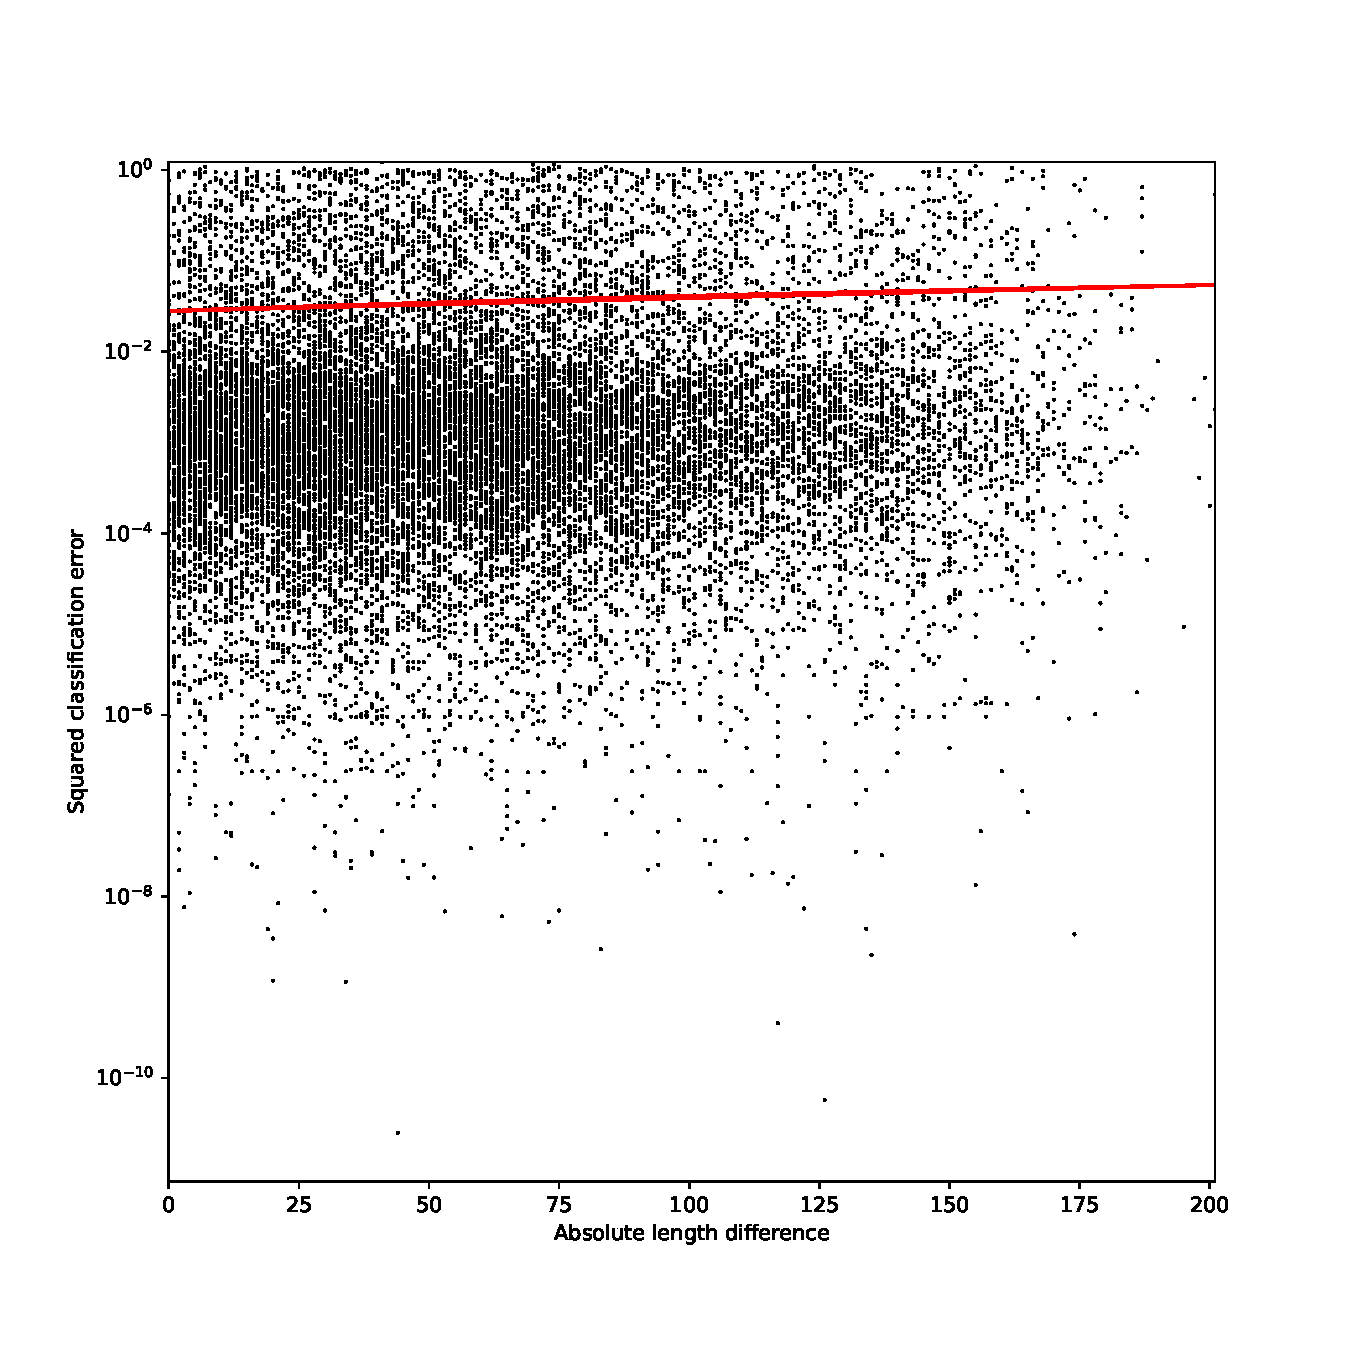
\includegraphics[width=\linewidth]{classification-error-length-difference-bert-train.pdf}
    \caption{Squared classification error for argument key point pairs from the validation set when matching with \BertBase. The horizontal axis shows the absolute length difference between the argument and the key point from each pair.}
    \label{classification-error-length}
\end{figure}
The same \BertBase matcher falsely predicts some argument key point pairs as non-matching.
For example, it seems to be very difficult to predict matches for the key point~7 \texttt{Affirmative action reduces quality.} from the topic \texttt{We should end affirmative action}, as shown in Figure~\ref{example-5-110-113}. These two arguments are longer than most arguments %\todo{from that topic?}
and especially longer than the key point.
It might be more challenging to reduce such longer arguments, containing more complex information, to very compact key points.
We confirm that observation by comparing the squared classification error with respect to the absolute difference between argument and key point lengths.
Figure~\ref{classification-error-length} shows that the more argument and key point differ in length, the greater the squared classification error gets when using the \BertBase matcher.
Comparable results can be observed for the \Roberta model.
We therefore identify length difference as a second general problem for both approaches.

% In contrast to \Bert, \Roberta performes way better when it comes to predicting non-matching pairs
% almost reproducing a similar performance as on the training set.
% \todo{Elaborate}

% \todo{Find example errors from our classifier. How can we improve?}
